\documentclass[border=5pt]{standalone}
\usepackage{tikz}
\usepackage{amsmath}
\usepackage{amssymb}
\usetikzlibrary{arrows.meta,calc,positioning}

\definecolor{ink}{HTML}{243142}
\definecolor{muted}{HTML}{667085}
\definecolor{vision}{HTML}{2E86AB}
\definecolor{model}{HTML}{E8871E}
\definecolor{policy}{HTML}{7FB069}

\begin{document}
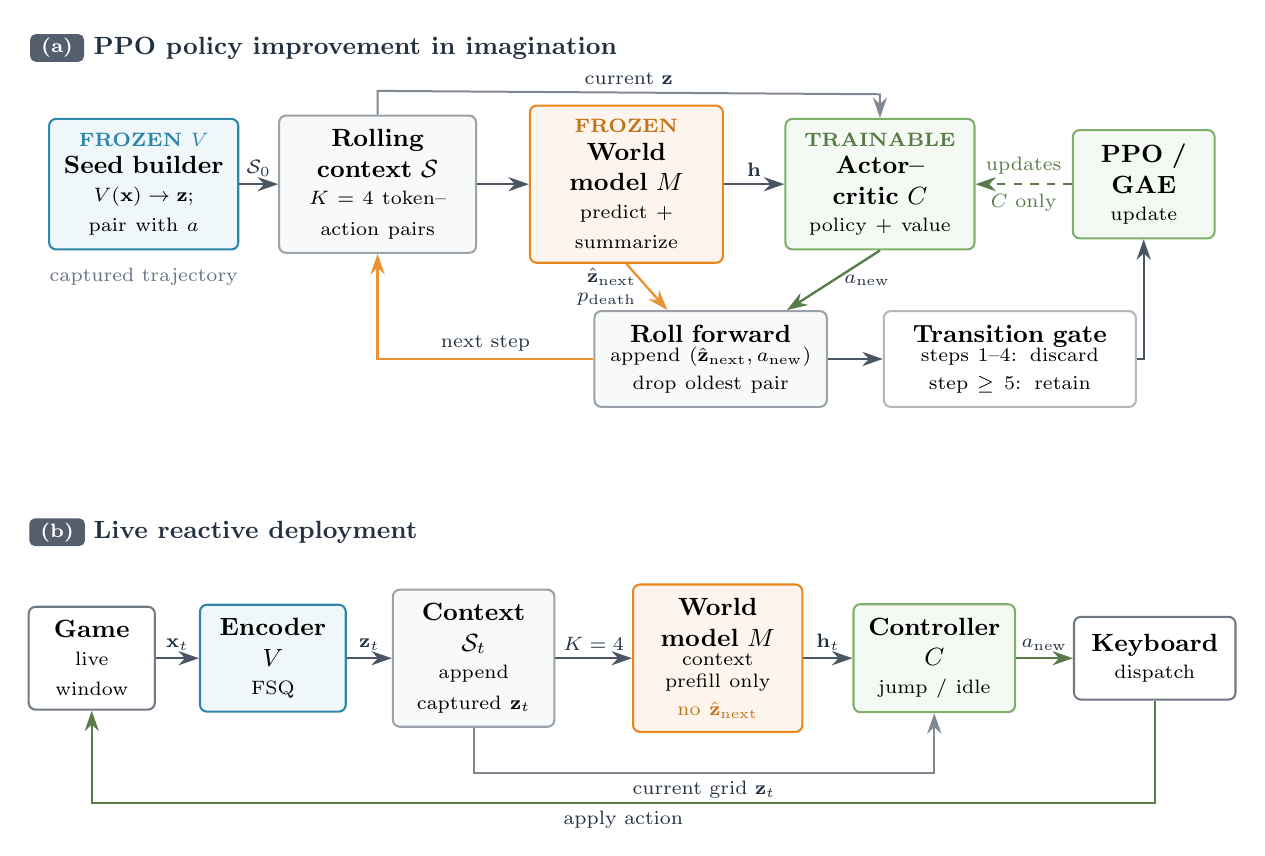
\begin{tikzpicture}[
  font=\sffamily,
  box/.style={
    rounded corners=2.5pt,
    draw=ink!65,
    line width=0.75pt,
    fill=white,
    minimum height=1.05cm,
    align=center,
    inner xsep=5pt,
    inner ysep=5pt,
    font=\small
  },
  visionbox/.style={box, draw=vision, fill=vision!7},
  contextbox/.style={box, draw=ink!45, fill=ink!3},
  modelbox/.style={box, draw=model, fill=model!8},
  policybox/.style={box, draw=policy, fill=policy!8},
  updatebox/.style={box, draw=ink!45, fill=ink!3},
  flow/.style={-{Stealth[length=2.6mm,width=1.8mm]}, line width=0.85pt, draw=ink!82},
  imagined/.style={flow, draw=model!90},
  policyflow/.style={flow, draw=policy!70!black},
  stateflow/.style={flow, draw=ink!58, line width=0.72pt},
  gradient/.style={-{Stealth[length=2.6mm,width=1.8mm]}, line width=0.85pt, draw=policy!70!black, dashed},
  edgelabel/.style={font=\scriptsize, text=ink, align=center, inner sep=0pt},
  note/.style={font=\scriptsize, text=muted, align=center},
  tag/.style={rounded corners=2pt, inner xsep=4pt, inner ysep=1.5pt, font=\scriptsize\bfseries, text=white, fill=ink!78},
]
  % (a) Offline policy improvement in imagination.
  \node[tag] at (-7.30,-0.35) {(a)};
  \node[anchor=west, font=\small\bfseries, text=ink] at (-6.96,-0.35)
    {PPO policy improvement in imagination};

  % Center the complete imagined-control pipeline beneath its heading.
  \begin{scope}[xshift=0.25cm,yshift=-0.18cm]
  \node[visionbox, text width=2.05cm] (seed) at (-6.45,-1.90)
    {{\scriptsize\bfseries\color{vision}FROZEN $V$}\\[-1pt]
     \textbf{Seed builder}\\[-1pt]
     \scriptsize $V(\mathbf x)\!\rightarrow\!\mathbf z$; pair with $a$};
  \node[note, below=0.10cm of seed] {captured trajectory};

  \node[contextbox, text width=2.15cm] (ctx) at (-3.48,-1.90)
    {\textbf{Rolling context $\mathcal S$}\\[-1pt]
     \scriptsize $K=4$ token--action pairs};
  \node[modelbox, text width=2.10cm] (wm) at (-0.32,-1.90)
    {{\scriptsize\bfseries\color{model!85!black}FROZEN}\\[-1pt]
     \textbf{World model $M$}\\[-1pt]
     \scriptsize predict + summarize};
  \node[policybox, text width=2.05cm] (ctrl) at (2.90,-1.90)
    {{\scriptsize\bfseries\color{policy!70!black}TRAINABLE}\\[-1pt]
     \textbf{Actor--critic $C$}\\[-1pt]
     \scriptsize policy + value};
  \node[policybox, text width=1.45cm] (ppo) at (6.25,-1.90)
    {\textbf{PPO / GAE}\\[-1pt]
     \scriptsize update};

  \node[updatebox, text width=2.60cm] (roll) at (0.75,-4.12)
    {\textbf{Roll forward}\\[-1pt]
     \scriptsize append $(\hat{\mathbf z}_{\rm next},a_{\rm new})$\\[-1pt]
     \scriptsize drop oldest pair};
  \node[box, draw=ink!35, text width=2.85cm] (gate) at (4.55,-4.12)
    {\textbf{Transition gate}\\[-1pt]
     \scriptsize steps 1--4: discard\\[-1pt]
     \scriptsize step $\geq5$: retain};

  \draw[flow] (seed) -- node[edgelabel, above=2.5pt] {$\mathcal S_0$} (ctx);
  \draw[flow] (ctx) -- (wm);
  \draw[flow] (wm) -- node[edgelabel, above=2.5pt] {$\mathbf h$} (ctrl);

  \coordinate (ctxrouteL) at ($(ctx.north)+(0,0.30)$);
  \coordinate (ctxrouteR) at ($(ctrl.north)+(0,0.30)$);
  \draw[stateflow] (ctx.north) -- (ctxrouteL)
    -- node[edgelabel, above=2.5pt] {current $\mathbf z$} (ctxrouteR)
    -- (ctrl.north);

  \draw[imagined] (wm.south) --
    node[edgelabel, pos=0.50, left=3.5pt, align=right]
      {$\hat{\mathbf z}_{\mathrm{next}}$\\[-1pt]$p_{\mathrm{death}}$}
    (roll);
  \draw[policyflow] (ctrl.south) --
    node[edgelabel, pos=0.50, right=3.5pt] {$a_{\mathrm{new}}$}
    (roll);

  \coordinate (rollturn) at (ctx.south |- roll.west);
  \draw[imagined] (roll.west) --
    node[edgelabel, above=2.5pt] {next step} (rollturn)
    -- (ctx.south);
  \draw[flow] (roll) -- (gate);
  \coordinate (gateturn) at (ppo.south |- gate.east);
  \draw[flow] (gate.east) -- (gateturn) -- (ppo.south);
  \draw[gradient] (ppo.west) --
    node[edgelabel, above=3pt, text=policy!70!black] {updates}
    node[edgelabel, below=3pt, text=policy!70!black] {$C$ only}
    (ctrl.east);
  \end{scope}

  % (b) Live reactive deployment.
  \node[tag] at (-7.30,-6.50) {(b)};
  \node[anchor=west, font=\small\bfseries, text=ink] at (-6.96,-6.50)
    {Live reactive deployment};

  % Account for the unequal widths of the Game and Keyboard edge modules so
  % the rendered deployment pipeline, rather than just their centers, is centered.
  \begin{scope}[xshift=-0.11cm]
  \node[box, text width=1.25cm] (game) at (-6.75,-8.10)
    {\textbf{Game}\\[-1pt]\scriptsize live window};
  \node[visionbox, text width=1.50cm] (enc) at (-4.45,-8.10)
    {\textbf{Encoder $V$}\\[-1pt]\scriptsize FSQ};
  \node[contextbox, text width=1.70cm] (livectx) at (-1.90,-8.10)
    {\textbf{Context $\mathcal S_t$}\\[-1pt]\scriptsize append captured $\mathbf z_t$};
  \node[modelbox, text width=1.80cm] (prefill) at (1.20,-8.10)
    {\textbf{World model $M$}\\[-1pt]
     \scriptsize context prefill only\\[-1pt]
     \scriptsize\color{model!85!black} no $\hat{\mathbf z}_{\mathrm{next}}$};
  \node[policybox, text width=1.70cm] (livectrl) at (3.95,-8.10)
    {\textbf{Controller $C$}\\[-1pt]\scriptsize jump / idle};
  \node[box, text width=1.70cm] (keys) at (6.75,-8.10)
    {\textbf{Keyboard}\\[-1pt]\scriptsize dispatch};

  \draw[flow] (game) -- node[edgelabel, above=2.5pt] {$\mathbf x_t$} (enc);
  \draw[flow] (enc) -- node[edgelabel, above=2.5pt] {$\mathbf z_t$} (livectx);
  \draw[flow] (livectx) -- node[edgelabel, above=2.5pt] {$K=4$} (prefill);
  \draw[flow] (prefill) -- node[edgelabel, above=2.5pt] {$\mathbf h_t$} (livectrl);
  \draw[policyflow] (livectrl) -- node[edgelabel, above=2.5pt] {$a_{\mathrm{new}}$} (keys);

  \coordinate (gridrouteL) at ($(livectx.south)+(0,-0.58)$);
  \coordinate (gridrouteR) at (livectrl.south |- gridrouteL);
  \draw[stateflow] (livectx.south) -- (gridrouteL)
    -- node[edgelabel, pos=0.50, below=2.5pt] {current grid $\mathbf z_t$} (gridrouteR)
    -- (livectrl.south);

  \coordinate (actionrouteR) at ($(keys.south)+(0,-1.30)$);
  \coordinate (actionrouteL) at (game.south |- actionrouteR);
  \draw[policyflow] (keys.south) -- (actionrouteR)
    -- node[edgelabel, below=2.5pt] {apply action} (actionrouteL)
    -- (game.south);
  \end{scope}

\end{tikzpicture}
\end{document}
